%!TEX root = ../dissertation.tex
% Insert PDF
% ex. 
\includepdf{figures/inserts/ch6.pdf}

\includepdf{figures/inserts/ch4.pdf}

% Set chapter number color to be similar to the insert color
\definecolor{chaptergrey}{rgb}{0.121148, 0.592739, 0.544641}
% Set citation number color to be similar to the insert color
\definecolor{SchoolColor}{rgb}{0.121148, 0.592739, 0.544641}

\thispagestyle{empty}
\begin{savequote}
    \normalfont\normalsize{P.T.A. Linders, E. Peters, M. ter Beest, and G. van den Bogaart\\}
\end{savequote}
\chapter{N-glycosylation is dependent on TMEM199-mediated V-ATPase assembly}
\addthumb{\thechapter}{\Large{\thechapter}}{white}{chaptergrey}
\stopthumb
\thispagestyle{empty}

\clearpage

\stopthumb
\section{Abstract}

The mammalian vacuolar H\textsuperscript{+}-ATPase (V-ATPase) is an important proton pump present at the membrane of the Golgi apparatus membrane and other organelles, where it ensures luminal pH suitable for Golgi processes. The molecular mechanisms of mammalian V-ATPase assembly are still unclear, but mutations in TMEM199, the mammalian homolog of yeast V-ATPase assembly factor Vma12p, cause a disorder of glycosylation characterized by hyposialylation, hypogalactosylation and elevated liver enzymes. In this study, we generate a HeLa cell model lacking TMEM199 with CRISPR/Cas9 to dissect the molecular mechanisms of disease. We observed that several enzymes responsible for glycosylation are mislocalized in TMEM199KO cells. Then, we applied a novel method to determine intraorganellar pH along the secretory pathway and observed that intraorganellar pH is misregulated in TMEM199KO cells. Finally, we performed biochemical studies to discover that TMEM199 is involved in the specific assembly of the Golgi- and endosome-localized V\textsubscript{0}a2 subunit and that TMEM199 is required for membrane association of CCDC115, the mammalian homolog of yeast V-ATPase assembly factor Vma22p. Thus, we present the underlying molecular mechanisms of glycosylation disorders caused by mutations in TMEM199.

\clearpage

\section{Introduction}

The Golgi apparatus has a well-defined pH gradient\cite{casey_sensors_2010} ranging from pH 6.7 at the \emph{cis}-Golgi to 6.0 at the \emph{trans}-Golgi\cite{casey_sensors_2010,kim_dynamic_1996,schapiro_determinants_2000,paroutis_ph_2004}. Not only is physiological pH required for proper folding, stability and function of proteins, at the Golgi apparatus pH is of utmost importance for the correct localization and activity of Golgi-localized glycosylation enzymes\cite{gawlitzek_ammonium_2000,linders_sugary_2020,fisher_bridging_2016,rivinoja_elevated_2009,maeda_chapter_2010}. Thus, strict maintenance of the Golgi pH gradient is critical and, in mammals, is in large part mediated by the vacuolar H\textsuperscript{+}-ATPase (V-ATPase).

The mammalian V-ATPase is a large multiprotein complex ($\approx$900 kDa) which acidifies intraorganellar lumina by translocating protons across the membrane\cite{forgac_vacuolar_2007,nishi_vacuolar_2002}. The V-ATPase can be subdivided into two separate domains: the membrane V\textsubscript{0} domain, consisting of six different subunits (a, d, e, c, c’, and c’’), which anchors the complex, and the cytosolic V\textsubscript{1} domain, consisting of eight different subunits (A-H), which hydrolyses ATP\cite{nishi_vacuolar_2002}. In mammals, four isoforms of the V\textsubscript{0}a subunit exist (V\textsubscript{0}a1-4), and this likely provides subcellular specificity with the V\textsubscript{0}a2 subunit primarily localizing to the Golgi apparatus and endosomes\cite{sun-wada_direct_2009,toyomura_lysosomes_2003,saw_vacuolar_2011,kornak_impaired_2008,pietrement_distinct_2006,hurtado-lorenzo_v-atpase_2006}. This is different from \emph{Saccharomyces cerevisiae} which only expresses two unique isoforms (Vph1p and Stv1p)\cite{forgac_vacuolar_2007,nishi_vacuolar_2002,kawasaki-nishi_amino-terminal_2001,kawasaki-nishi_yeast_2001,manolson_stv1_1994}.

Assembly of the V\textsubscript{0} domain in yeast is dependent on a set of ER-localized chaperones: Vma12p, Vma21p and Vma22p\cite{forgac_vacuolar_2007,graham_assembly_1998,hill_vma22p_1995,jackson_vma12_1997,malkus_role_2004}. Mammalian homologues of Vma12p (TMEM199), Vma21p (VMA21) and Vma22p (CCDC115) have recently been identified and genetic variants in these proteins are associated with disorders of glycosylation\cite{jansen_tmem199_2016,jansen_ccdc115_2016,cannata_serio_mutations_2020}. Moreover, TMEM199 and CCDC115 have been shown to interact and are important for physiological iron homeostasis, a process that also relies on intraorganellar pH\cite{miles_vacuolar-atpase_2017}. However, their role in mammalian V-ATPase assembly is poorly understood.

In this study, we dissected the role of TMEM199 in mammalian V-ATPase assembly. We developed a HeLa cell line deficient of TMEM199 by CRISPR/Cas9 and, using a novel method for intraorganellar pH measurements, measured the effect of the knockout on intracellular pH. To prove that TMEM199 is indeed an assembly factor of the mammalian V-ATPase, we performed fractionation studies and examined whether TMEM199 can tether CCDC115 to the membrane.

\section{Results}

\subsection{Generation of a TMEM199KO model}

To study the role of TMEM199 in glycosylation and V-ATPase assembly, we generated two unique partial TMEM199 knockout HeLa cell lines from the same gRNA (B1 and B2; Figure~\ref{fig:ch4fig1}a), with different levels of residual TMEM199 expression, using CRISPR/Cas9. 
To confirm that these knockout models are suitable to study the glycosylation defects observed in TMEM199-CDG patients\cite{jansen_tmem199_2016}, we performed cell surface staining with the SNA-I lectin from \emph{Sambucus nigra}, which binds terminal sialic acid moieties in an $\alpha$-2,6 linkage and to a lesser extent $\alpha$-2,3 linkage of N-glycans. Compared to parental HeLa cells, we observed an approximate 60\% decrease in SNA-I labeling for both TMEM199KO clones (Figure~\ref{fig:ch4fig1}b, c, flow cytometry gating strategy in Supplementary Figure~\ref{fig:ch4supfig1}). As TMEM199-CDG patients present with a similar decrease in sialylation\cite{jansen_tmem199_2016}, we concluded from this experiment that our TMEM199KO clones are a suitable model for the glycosylation defect.

\begin{figure}
    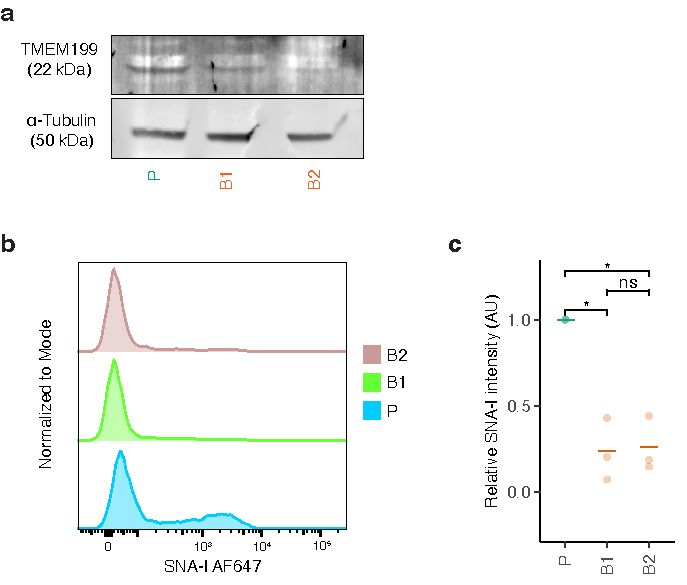
\includegraphics[keepaspectratio=true]{chapters/chapter4/chapter4_Figure1.pdf}
    \caption{\textbf{TMEM199KO HeLa cell lines show defective cell surface sialylation.} \textbf{(a)} Representative immunoblot for TMEM199 on cell lysates of parental HeLa cells (P, green) or TMEM199KO cells (B1 and B2, orange). $\alpha$-Tubulin, loading control. \textbf{(b)} Representative FACS histogram of parental HeLa cells (blue, P), or two TMEM199KO lines (green, B1 and pink, B2), probed with SNA-I lectin conjugated to Alexa Fluor 647. Gating strategy in Supplementary Figure~\ref{fig:ch4supfig1}. \textbf{(c)} Quantification of (b). Geometric means were taken and normalized to parental. 10,000 events analyzed per condition per experiment from 3 independent experiments.}
    \label{fig:ch4fig1}
\end{figure}

\subsection{Loss of TMEM199 relocalizes glycosyltransferases}

Given that our TMEM199KO cell models have defective cell surface glycosylation, we investigated whether there is a potential trafficking defect by probing for the localization of glycosyltransferases in the Golgi apparatus. We performed immunofluorescence labeling of mannosyl ($\alpha$-1,3)-glycoprotein $\beta$-1,2-N-acetylglucosaminyltransferase (MGAT1, also known as GnT1), which catalyzes the addition of N-acetylglucosamine (GlcNAc) to the early Golgi-related glycan man-5. Compared to parental HeLa cells, TMEM199KO B1 showed a slightly increased colocalization of MGAT1 with \emph{cis}-Golgi marker GM130 (Figure~\ref{fig:ch4fig2}a, b) and \emph{trans}-Golgi marker TGN46 (Figure~\ref{fig:ch4fig2}c, d), while TMEM199KO B2 shows a strongly decreased colocalization of MGAT1 with GM130 and a slightly increased colocalization with TGN46. As TMEM199-CDG patients show hypogalactosylation, we next investigated the localization of $\beta$-1,4-galactosyltransferase 1 (B4GALT1, also known as GalT) which catalyzes the addition of galactose to N-acetylglucosamine moieties (Supplementary Figure~\ref{fig:ch4supfig2}). Compared to parental HeLa cells, we observed a decrease of B4GALT1 colocalization with \emph{cis}-Golgi marker ZFPL1\cite{chiu_zfpl1_2008} in B1 cells, but an increase in ZFPL1 colocalization in B2 cells. For TGN46 colocalization, no difference was observed for B1 cells but we observed a decrease in colocalization in B2 cells. Finally, N-acetylgalactosaminyltransferase 2 (GALNT2), which catalyzes the first step in mucin O-linked glycan synthesis, located slightly more to the \emph{cis}-Golgi (marker ZFPL1), and slightly less to \emph{trans}-Golgi (marker TGN46) in B2 cells (Supplementary Figure~\ref{fig:ch4supfig3}).

\begin{figure}
    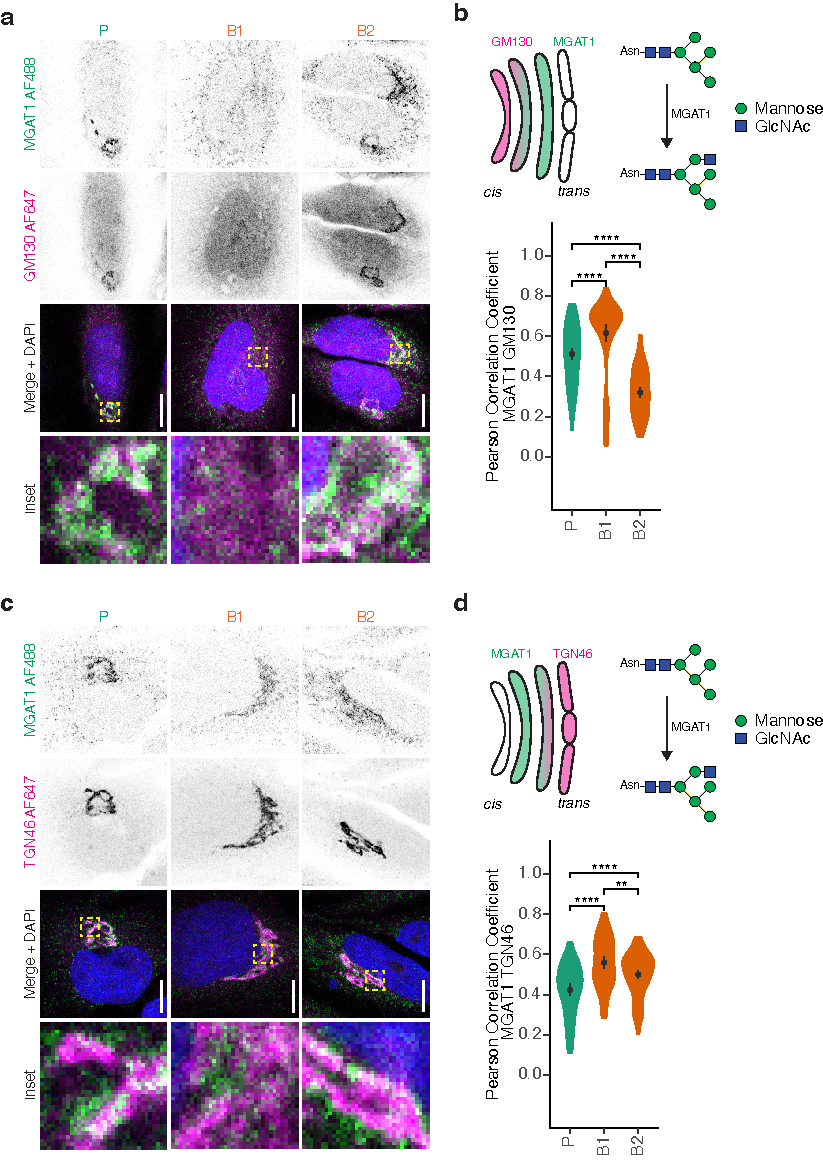
\includegraphics[keepaspectratio=true,width=\textwidth,height=\textheight]{chapters/chapter4/chapter4_Figure2.pdf}
    \caption{\textbf{Relocation of glycosyltransferase MGAT1 in TMEM199KO HeLa cells.} (Continued on the following page.)}
    \label{fig:ch4fig2}
\end{figure}
\begin{figure}[t]
    \contcaption{\textbf{(a)} Immunofluorescence microscopy of MGAT1 (green in merge) and GM130 (magenta) in parental HeLa cells (green, P) or TMEM199KO cells (B1 and B2, orange). Representative confocal micrographs. Scalebars, 10 $\mu$m. DAPI in blue. \textbf{(b)} Pearson’s correlation coefficients between MGAT1 and GM130 of panel (a). N = 118 (P), 78 (B1), and 99 (B2) from two independent experiments. \textbf{(c)} Same as panel (a) but now for MGAT1 (green) and TGN46 (magenta). \textbf{(d)} Pearson’s correlation coefficients between MGAT1 and TGN46 of panel (c). N = 75 (P), 68 (B1), and 99 (B2) from two independent experiments.}
\end{figure}

As a control, we investigated protein expression levels (inferred from the fluorescence intensity of the immunofluorescence labeling) of the markers used in the colocalization experiments, and did not find a correlation between expression and differences in colocalization (Supplementary Figure~\ref{fig:ch4supfig4}). We did observe a slight condensation of GM130 labeling area in B1 cells and a slight dilation in B2 cells, while we observed condensation of ZFPL1 labeling area only in B2 cells. A similar condensation phenotype was observed for TGN46 in B2 cells. These results suggest that the Golgi morphology is differentially altered in the two TMEM199 knockout strains.

Taken together, and despite the partially opposite phenotypes in the two TMEM199 knockout strains, the (partial) loss of TMEM199 causes the aberrant localization of glycosyltransferases to the Golgi apparatus and slight morphological differences of the Golgi. Computational simulations have shown that disruption of Golgi structure and mislocalization of glycosyltransferases can have a profound impact on glycosylation\cite{jaiman_golgi_2020}.

\subsection{pH measurements in TMEM199KO cells}

As TMEM199 is a supposed V-ATPase assembly factor and physiological pH homeostasis is necessary to maintain the delicate structure of the Golgi5–9, we then investigated whether the aberrant localization of glycosyltransferases is caused by defective Golgi lumen pH regulation. We applied our earlier developed method based on the fusion of a pH-sensitive GFP mutant, ratiometric pHLuorin2\cite{mahon_phluorin2:_2011,miesenbock_visualizing_1998}, to organellar markers to measure intraorganellar pH using fluorescence lifetime imaging microscopy (FLIM)\cite{linders_fluorescence_2021} (Figure~\ref{fig:ch4fig3}). We measured an ER luminal pH of 7.4 for parental HeLa cells, which was strongly decreased for B1 cells (pH 6.7) and even further decreased in B2 cells (pH 6.5) (Figure~\ref{fig:ch4fig3}a, b). Golgi pH was slightly decreased as measured by MGAT2-RpHLuorin2 (\emph{cis}/medial-Golgi, P: pH 6.3, B1: pH 6.1, B2: pH 6.1; Figure~\ref{fig:ch4fig3}c, d) and GalT-RpHLuorin2 (\emph{trans}-Golgi, P: pH 6.4, B1: pH 6.0, B2: pH 5.9; Figure~\ref{fig:ch4fig3}e, f). Finally, we observed no significant difference between parental cells and B1 cells in lysosomal pH as measured by LAMP1-RpHLuorin2 (P: pH 5.0, B1: pH 4.9; Figure~\ref{fig:ch4fig3}g, h) but we measured a decrease in lysosomal pH for B2 cells (pH 4.5; Figure~\ref{fig:ch4fig3}g, h). We expected that a dysfunctional V-ATPase assembly in TMEM199KO would result in an increased intraorganellar pH due to defective acidification. However, our results contrast this hypothesis as we observed stronger acidification along the entire secretory pathway.

\begin{figure}
    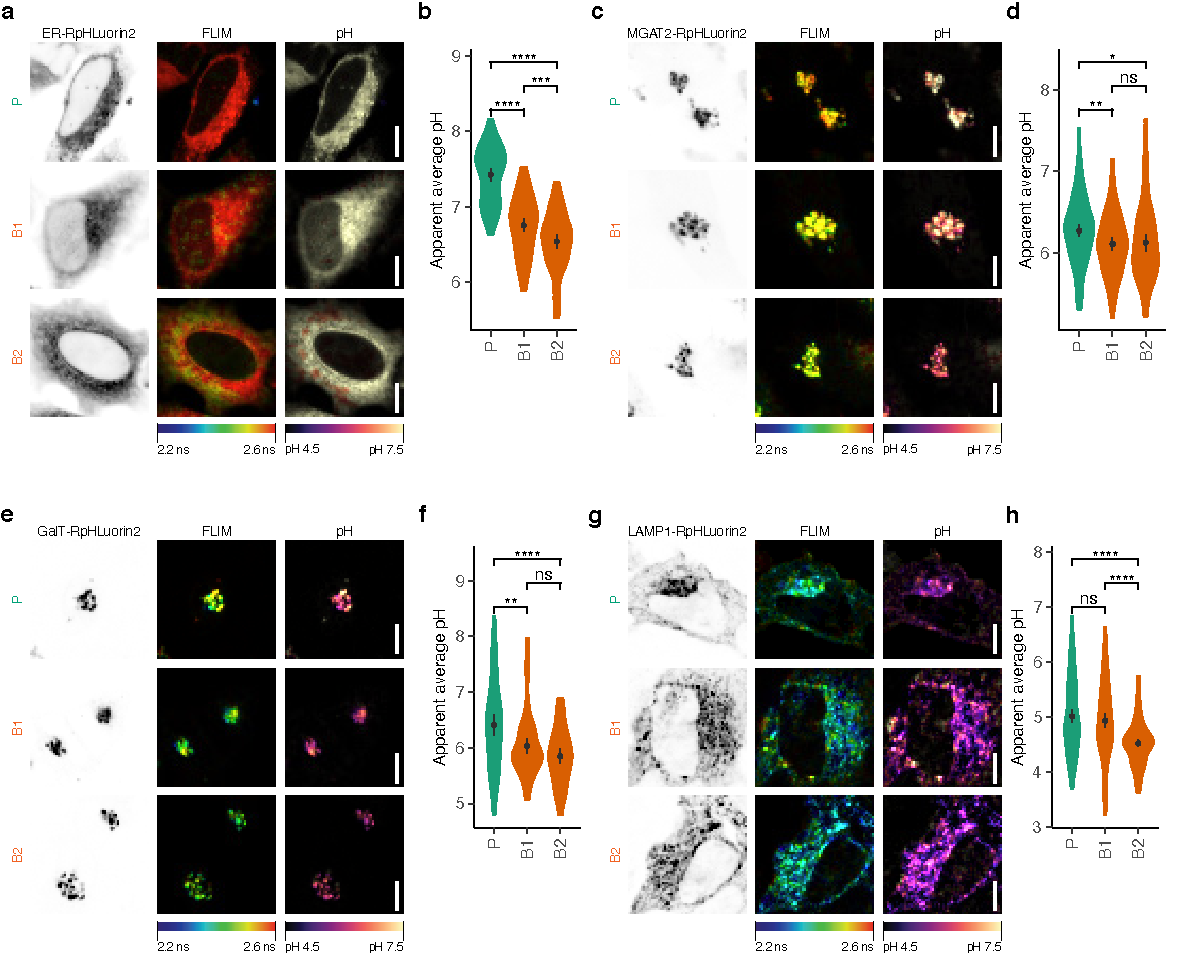
\includegraphics[keepaspectratio=true,width=\textwidth,height=\textheight]{chapters/chapter4/chapter4_Figure3.pdf}
    \caption{\textbf{Decreased luminal pH in TMEM199KO HeLa cells.} \textbf{(a)} Representative confocal micrographs of parental HeLa cells (P, green) or TMEM199KO cells (B1 and B2, orange) expressing ER-RpHLuorin2. The intensity image (left column) was convoluted with the fluorescence lifetime value (middle column) and the calculated pH (right column) per pixel. FLIM, fluorescence lifetime imaging microscopy. Scalebars, 10 $\mu$m. \textbf{(b)} Quantification of average pH values from panel (a). N = 79 (P), 80 (B1), and 80 (B2) from 3 independent experiments. \textbf{(c)} Same as panel (a) but now for MGAT2-RpHLuorin2. \textbf{(d)} Quantification of average pH values from panel (c). N = 117 (P), 97 (B1), and 72 (B2) from 3 independent experiments. \textbf{(e)} Same as panel (a) but now for GalT-RpHLuorin2. \textbf{(f)} Quantification of average pH values from panel (e). N = 65 (P), 72 (B1), and 52 (B2) from 3 independent experiments. \textbf{(g)} Same as panel (a) but now for LAMP1-RpHLuorin2. \textbf{(h)} Quantification of average pH values from panel (g). N = 123 (P), 111 (B1), and 147 (B2) from 3 independent experiments.}
    \label{fig:ch4fig3}
\end{figure}

As the observed misregulation of pH might already mislocalize the probes we applied to measure intraorganellar pH, it is possible that the localization of the probes in the B1 and B2 cells does not reflect the same localization as in the parental cells. Thus, we developed a different strategy for assessing V-ATPase activity by measuring intraorganellar pH in the absence or presence of the V-ATPase inhibitor Bafilomycin A1 (BafA1)\cite{huss_inhibitors_2009}. We reasoned that if less V-ATPase molecules are present in organellar membranes, the difference in luminal pH ($\Delta$pH) between BafA1-treated cells and the DMSO control should be lower. For ER-RpHLuorin2 expressed in parental HeLa cells, we measured a lower luminal pH when treated with only DMSO compared to our previous measurements (pH 6.4 with DMSO compared to pH 7.4; Figure~\ref{fig:ch4fig4}a, Supplementary Figure~\ref{fig:ch4supfig5}a), likely as a result of DMSO treatment, and this increased to pH 6.5 when incubated with 200 nM BafA1. Similar results with DMSO were observed for the B1 and B2 cells (pH 6.3 and pH 6.1 respectively), but $\Delta$pH was slightly decreased in B1 cells compared to parental HeLa, but somewhat increased in B2 cells (Figure~\ref{fig:ch4fig4}a, b, Supplementary Figure~\ref{fig:ch4supfig5}a). We observed similar results for \emph{cis}-/medial-Golgi marker MGAT2-RpHLuorin2, where $\Delta$pH was significantly decreased for B1 cells but slightly increased for B2 cells (Figure~\ref{fig:ch4fig4}c, d, Supplementary Figure~\ref{fig:ch4supfig5}b). Finally, we performed the same assay for \emph{trans}-Golgi marker GalT-RpHLuorin2. Here we observed a small increase in $\Delta$pH for B1 cells but BafA1-sensitivity was absent for B2 cells (Supplementary Figure~\ref{fig:ch4supfig5}c-e). The observed increase in $\Delta$pH for the B2 cells in both ER and early Golgi compartments does not support a role of TMEM199 in V-ATPase assembly but suggests aberrant trafficking and/or processing of the V-ATPase as more V-ATPase molecules appear to be present on the ER membrane. Concurrently, less V-ATPase might be present on GalT-positive compartments which could indicate a disorganization of the pH gradient in the secretory pathway.

\begin{figure}
    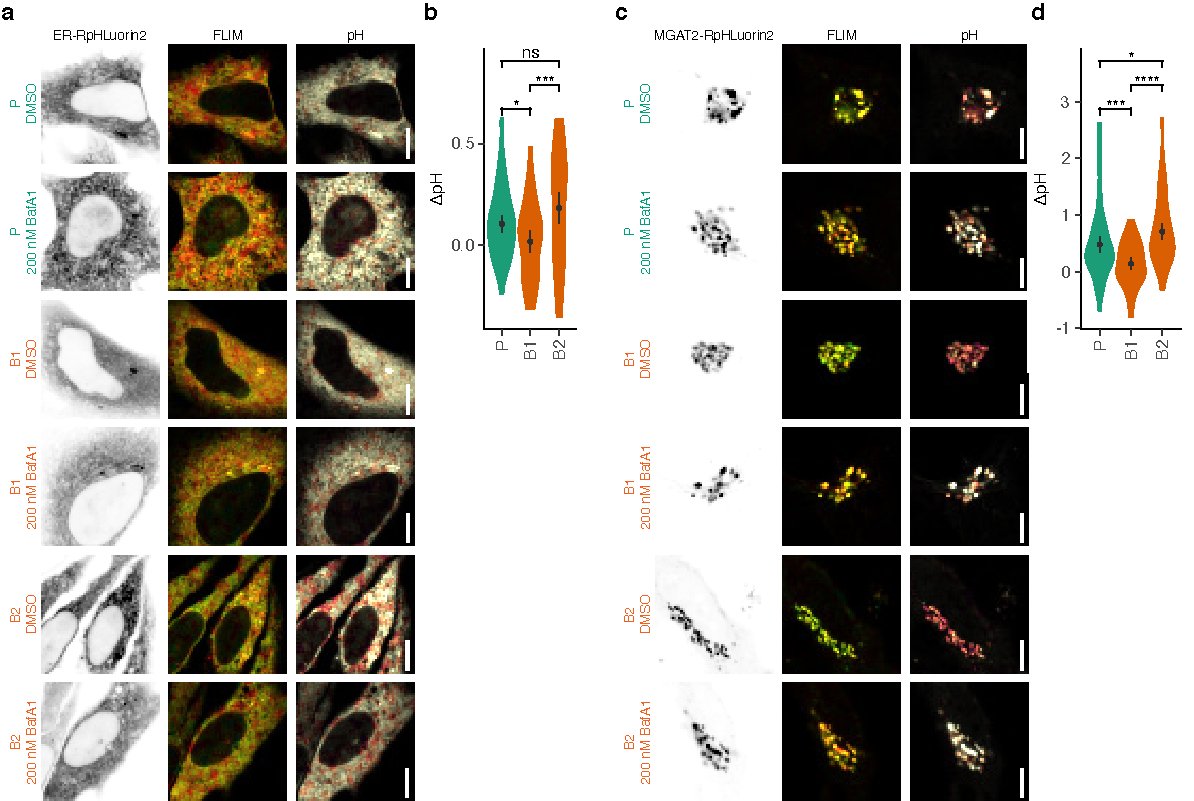
\includegraphics[keepaspectratio=true,width=\textwidth,height=\textheight]{chapters/chapter4/chapter4_Figure4.pdf}
    \caption{\textbf{FLIM-based pH measurements in TMEM199KO HeLa cells challenged with V-ATPase inhibitor Bafilomycin A1.} \textbf{(a)} Representative confocal micrographs of parental HeLa cells (P, green) or TMEM199KO cells (B1 and B2, orange), in the absence (DMSO) or presence of Bafilomycin A1 (200 nM BafA1). The intensity image (left column) was convoluted with the fluorescence lifetime value (middle column) and the calculated pH (right column) per pixel. FLIM, fluorescence lifetime imaging microscopy. Scalebars, 10 $\mu$m. \textbf{(b)} Quantification of the difference in pH ($\Delta$pH) between vehicle control (DMSO) and cells challenged with Bafilomycin A1 from panel (a). N = 84 (P, DMSO), 62 (P, 200 nM BafA1), 41 (B1, DMSO), 46 (B1, 200 nM BafA1), 43 (B2, DMSO), and 50 (B2, 200 nM BafA1) from 2 independent experiments. \textbf{(c)} Same as panel (a) but now for MGAT2-RpHLuorin2. \textbf{(d)} Quantification of the difference in pH ($\Delta$pH) between vehicle control (DMSO) and cells challenged with Bafilomycin A1 from panel (c). N = 72 (P, DMSO), 77 (P, 200 nM BafA1), 78 (B1, DMSO), 46 (B1, 200 nM BafA1), 63 (B2, DMSO), and 71 (B2, 200 nM BafA1) from 2 independent experiments.}
    \label{fig:ch4fig4}
\end{figure}

\subsection{Biochemical investigations of the role of TMEM199 in V-ATPase assembly}

Prior to V\textsubscript{0} – V\textsubscript{1} assembly, the V\textsubscript{0} domain is first assembled in the ER\cite{forgac_vacuolar_2007,esmail_n-linked_2016,esmail_n-linked_2017,ramachandran_vma21_2013}. Previous studies have shown that the stability of the V\textsubscript{0}a subunits is dependent on this assembly of the V\textsubscript{0} domain, resulting in degradation of the V\textsubscript{0}a subunits when the V\textsubscript{0} domain is not assembled\cite{esmail_n-linked_2016,esmail_n-linked_2017}. We investigated the stability of endogenous V\textsubscript{0}a1-3 in the parental HeLa cells and the B1 and B2 cells when chased with ribosomal inhibitor cycloheximide (Figure~\ref{fig:ch4fig5}a-d). Stability of the subunits V\textsubscript{0}a1 and V\textsubscript{0}a3 was not visibly altered between parental HeLa cells, B1 and B2 cells (Figure~\ref{fig:ch4fig5}a, b, d). However, we did observe lower stability of the Golgi- and endosome-localized V\textsubscript{0}a2 subunit in both TMEM199 knockout strains (Figure~\ref{fig:ch4fig5}a, c), suggesting that TMEM199 might be involved in the assembly of a Golgi- and endosome-specific V\textsubscript{0}-domain.

\begin{figure}
    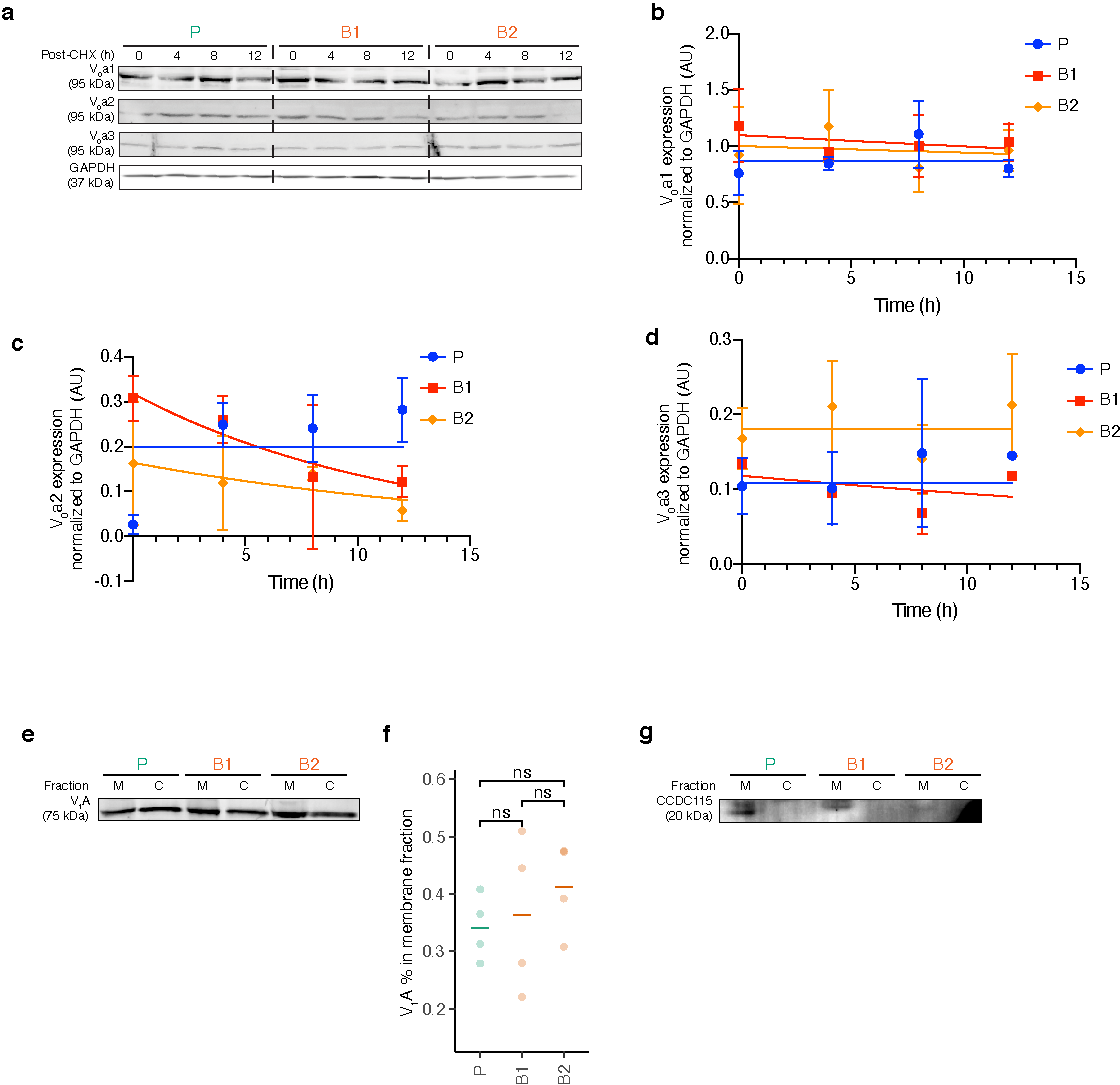
\includegraphics[keepaspectratio=true,width=\textwidth,height=\textheight]{chapters/chapter4/chapter4_Figure5.pdf}
    \caption{\textbf{The role of TMEM199 in mammalian V-ATPase assembly.} \textbf{(a)} Representative immunoblot of cell lysates for the stability of V-ATPase subunits V\textsubscript{0}a1, V\textsubscript{0}a2, and V\textsubscript{0}a3, in parental HeLa cells (P, green) or TMEM199KO cells (B1 and B2, orange) treated with cycloheximide (CHX) for the times indicated. GAPDH, loading control. \textbf{(b)} Quantification of panel (a) for V\textsubscript{0}a1. Protein expression levels were normalized to GAPDH signal. Data from 2 independent experiments. \textbf{(c)} Same as panel (b) but now for V\textsubscript{0}a2. \textbf{(d)} Same as panel (b) but now for V\textsubscript{0}a3. \textbf{(e)} Representative immunoblot of V-ATPase subunit V\textsubscript{1}A in membrane (M) and cytosolic (C) fractions of cell lysates from parental HeLa cells (P, green) or TMEM199KO cells (B1 and B2, orange) after crosslinking with DSP. Membrane and cytosolic fractions were obtained by ultracentrifugation. \textbf{(f)} Quantification of panel (e). Each point represents the percentage of the V\textsubscript{1}A membrane fraction, obtained by dividing the membrane signal by the total V1A signal (membrane + cytosolic fraction) from one experiment. Data from 4 independent experiments. \textbf{(g)} Representative immunoblot of CCDC115 in membrane (M) and cytosolic (C) fractions of cell lysates from parental HeLa cells (P, green) or TMEM199KO cells (B1 and B2, orange) after crosslinking with DSP. Membrane and cytosolic fractions were obtained by ultracentrifugation.}
    \label{fig:ch4fig5}
\end{figure}

To investigate whether these results have any implication on overall V\textsubscript{0} – V\textsubscript{1} assembly, we fractionated parental HeLa, B1 and B2 cells into membrane and cytosolic fractions following intracellular crosslinking with dithiobis(succinimidyl propionate) (DSP) (Figure~\ref{fig:ch4fig5}e, f). We then quantified the relative amounts of the V\textsubscript{1}A subunit from the cytosolic V\textsubscript{1} domain present in the membrane fraction and observed an unsignificant trend towards more overall V\textsubscript{0} – V\textsubscript{1} assembly in the TMEM199KO cells. These results suggest that although less V\textsubscript{0}a2-specific assembly might occur, complete V-ATPase assembly might be somewhat increased.

Finally, as it is known that cytosolic CCDC115 can interact with the integral membrane protein TMEM199\cite{miles_vacuolar-atpase_2017}, we investigated whether CCDC115 would be associated with the membrane fractions. From yeast it is understood that cytosolic Vma22p can associate with membrane Vma12p\cite{graham_assembly_1998} and this interaction is required for V-ATPase assembly in yeast. Thus, we hypothesized that a similar interaction is important in mammalian cells and that the loss of TMEM199 should cause less membrane association of CCDC115. We interrogated the presence of CCDC115 in the earlier obtained DSP-treated membrane fractions and we observed slightly less CCDC115 in the membrane fraction of B1 cells, and almost no CCDC115 in the membrane fraction of B2 cells (Figure~\ref{fig:ch4fig5}g). We did not observe CCDC115 in the cytosolic fraction, which could be an indication of cytosolic instability of CCDC115. Taken together, these results suggest that TMEM199 might be important for the specific assembly of a V\textsubscript{0}a2-containing V-ATPase, possibly together with CCDC115.

\clearpage

\section{Discussion}

In this study, we investigated the function of TMEM199 in intraorganellar acidification. The yeast homolog of TMEM199, Vma12p, is a known assembly factor of the V-ATPase\cite{graham_assembly_1998,jackson_vma12_1997} and is thereby involved in luminal pH maintenance. Our findings suggest a specific role for TMEM199 in assembly of V\textsubscript{0}a2-containing V-ATPase, but not or less V-ATPases with the other three V\textsubscript{0}a subunits in mammalian cells\cite{sun-wada_direct_2009,toyomura_lysosomes_2003,saw_vacuolar_2011,kornak_impaired_2008,pietrement_distinct_2006,hurtado-lorenzo_v-atpase_2006}. This specific role seems to contrast yeast where Vma12p has a more general function in V-ATPase assembly\cite{graham_assembly_1998,jackson_vma12_1997}.

In some of our experiments, we observed opposite phenotypes for the two TMEM199KO strains: the subcellular localization of glycosyltransferases and the pH measurements upon Bafilomycin A1 treatment were significantly altered in opposite directions for the two strains. This might be a consequence of off-target effects of the gRNA in one of these strains. Alternatively, the contrasting phenotypes could be caused by the different residual expression of TMEM199, as strain B1 had somewhat higher levels of TMEM199 than B2. This might result in differences of residual V-ATPase activity and cause the different luminal pH values and subcellular localization of the glycosyltransferases. Moreover, Golgi pH is not only regulated by the V-ATPase, but partly also by passive backflux of H\textsuperscript{+} ions and by ion channels such as GPHR\cite{maeda_gphr_2008}. The activity and/or localization of these factors might also be sensitive to the levels of V-ATPase activity, and thereby contribute to the different phenotypes observed in the two TMEM199KO strains.

TMEM199 has been shown to mediate the V\textsubscript{0} – V\textsubscript{1} assembly in human lung adenocarcinoma A549 cells\cite{li_genome-wide_2020}. However, we were not able to observe this with our TMEM199 knockout HeLa models but instead mostly observed a lower intraorganellar pH, suggesting elevated V-ATPase activity, at the ER and early Golgi compartments. The regulation and function of the V-ATPase is altered in different kinds of tumor cells\cite{stransky_function_2016} and this might explain the differences observed between HeLa cells and A549 cells lacking TMEM199. An important finding is the specific degradation of V\textsubscript{0}a2 in TMEM199-lacking cells. Therefore, a possible explanation for the discrepancy between our study and previous findings in A549 cells\cite{li_genome-wide_2020}, could be that A549 cells are more dependent on the V\textsubscript{0}a2-defined V-ATPase and are therefore more sensitive to the loss of TMEM199. HeLa cells might then be more dependent on other V\textsubscript{0}a subunits, meaning the loss of the V\textsubscript{0}a2-defined V-ATPase would not result in a loss of acidification.

However, we even observed an increased acidification in the ER and early Golgi compartments in HeLa cells lacking TMEM199, suggesting that there is more V-ATPase present on these organellar membranes upon loss of TMEM199. This conclusion was strengthened by the increased sensitivity of ER-localized V-ATPase to Bafilomycin A1 in one of the TMEM199KO strains. One possibility for the increased luminal acidification in TMEM199KO is that there might be increased assembly of V-ATPases, perhaps as a compensatory mechanism for the reduction of the V\textsubscript{0}a2-containing V-ATPase. Another possibility is that TMEM199 is involved in the trafficking of the V-ATPase from the ER to other organelles, and lack of TMEM199 results in elevated levels and activity of the V-ATPase in the ER and early Golgi compartments.

The fractionation studies we presented in this study revealed a potential molecular mechanism for the phenotypes observed in TMEM199-CDG patients\cite{jansen_tmem199_2016}. Our results suggest that CCDC115 is recruited to membranes by TMEM199. Mutations in both CCDC115 and TMEM199 are a cause of glycosylation disorders, although the pathological condition in TMEM199-CDG seem more limited (mostly hepatological involvement)\cite{jansen_tmem199_2016}, while CCDC115-CDG is characterized by more severe symptoms including neurological involvement\cite{jansen_ccdc115_2016}. An explanation for this difference could be that there is another mechanism for CCDC115 to exert its function in absence of TMEM199. Another, more likely, explanation is that the genetic variants found in TMEM199-CDG patients still produce TMEM199 protein, but that the binding affinity with for instance CCDC115 is reduced. This might result in a milder phenotype for TMEM199-CDG than for CCDC115-CDG.

\subsection{Acknowledgments}

We thank Feng Zhang for providing the eSpCas9(1.1) construct (Addgene plasmid \#71814). We also thank the Microscopic Imaging Center of the Radboud Institute for Molecular Life Sciences for use of their microscopy facilities. G.v.d.B. is funded by a Young Investigator Grant from the Human Frontier Science Program (HFSP; RGY0080/2018) and a Vidi grant from the Netherlands Organisation for Scientific Research (NWO-ALW VIDI 864.14.001). G.v.d.B has also received funding from the European Research Council (ERC) under the European Union’s Horizon 2020 research and innovation program (grant agreement No. 862137).

\subsection{Author Contributions}

P.T.A.L., E.P., M.t.B., and G.v.d.B. designed and performed the experiments and wrote the paper.

\subsection{Declaration of Interests}

The authors declare that they have no competing financial interests.

\clearpage

\section{Methods}

\subsection{Cell culture and transfection}

HeLa cells (authenticated by ATCC through their human STR profiling cell authentication service) and derived TMEM199KO cells were maintained in high glucose DMEM with Glutamax (Gibco 31966021), supplemented with 10\% fetal calf serum (FCS, Greiner Bio-one, Kremsmünster, Austria) and antibiotic-antimycotic solution (Gibco 15240-062). Cells were regularly tested for mycoplasma contamination. Cells were transfected with plasmid vectors using Fugene HD (Promega E2311), using the recommended protocol of the manufacturer. Cells were processed 48 hours post-transfection. Only cells expressing low to moderate levels of the transfected plasmids, based on fluorescence intensity and manual localization scoring, were chosen for subsequent microscopic analyses.

\subsection{Antibodies}

The following primary antibodies and dilutions were used in this study: rabbit polyclonal anti-TMEM199 (Novus Biological, NBP1-88467, 1:250), rat monoclonal anti-$\alpha$-Tubulin (YOL1/34, Novus Biologicals NB100-1639, 1:2000) rabbit monoclonal anti-MGAT1 (Abcam, ab180578, 1:100), mouse monoclonal anti-GALNT2 (1501421, Biolegend 682302, 1:100), mouse monoclonal anti-B4GALT1 (GT2/36/118, Enzo ALX-803-339-c050, 1:100), mouse monoclonal anti-GM130 (35/GM130, BD Transduction Laboratories 610822, 1:100), rabbit polyclonal anti-ZFPL1 (Sigma HPA014909, 1:100), sheep polyclonal anti-TGN46 (BioRad AHP500GP, 1:1000), rabbit monoclonal anti-GAPDH (14C10, Cell Signaling Technology 2118, 1:2000), rabbit polyclonal anti-V\textsubscript{0}a1 (Novus Biological NBP1-89342, 1:500), rabbit polyclonal anti-V\textsubscript{0}a2 (Novus Biological NBP1-59069, 1:500), mouse monoclonal anti-V\textsubscript{0}a3 (Novus Biological H00010312-M01, 1:500), mouse monoclonal anti-V\textsubscript{1}A (4F5, Santa Cruz Biotechnology sc-293336, 1:500), and rabbit polyclonal anti-CCDC115 (Proteintech, 20636-1-AP, 1:250).

\subsection{CRISPR/Cas9}

Knockout of TMEM199 in HeLa cells was achieved using CRISPR/Cas9. We used the prior described gRNA sequence: 5’ – TATGG CGTCC TCTTT GCTTG CGG\cite{miles_vacuolar-atpase_2017}. The gRNA sequence was cloned in eSpCas9(1.1) (Gift from Feng Zhang, Addgene no. 71814)\cite{slaymaker_rationally_2016} and transfected into HeLa cells by Fugene HD (Promega). 72 hrs after transfection, the medium of puromycin-resistant cells was changed for conditioned medium (collected from parental HeLa cells at 70\% confluency) supplemented 1:1 with fresh medium. Single clones were obtained and screened for knockout of TMEM199 by SDS-PAGE and Western blotting and finally validated by Sanger sequencing. Residual TMEM199 might be a consequence of contamination by parental HeLa cells during cell culture.

\subsection{Lectin stainings}
Cells were plated in 6-well plates and incubated until confluent ($\approx$72 h). Cells were released from the culture substrate with 2 mM EDTA in PBS. Cells were then blocked with Carbo-Free blocking solution (Vector Laboratories, SP-5040) and incubated with and incubated with 4 $\mu$g/mL biotinylated SNA-I (Vector Laboratories, B-1305) diluted in Carbo-Free Blocking solution. Cells were then incubated with Streptavidin-Alexa Fluor 647 (ThermoScientific, S32357) and finally resuspended in FACS buffer (phosphate buffered saline + 0.5\% FBS + 0.01\% NaN\textsubscript{3}), supplemented with 300 ng/mL 4′,6-diamidino-2-phenylindole (DAPI) for live/dead discrimination. Samples were run on a FACSLyric flow cytometer (BD Biosciences) and analyzed with FlowJo X (FlowJo, LLC).

\subsection{pH measurements}

pH measurements were performed as described previously\cite{linders_fluorescence_2021}. Briefly, RpHLuorin2-tagged constructs were transiently overexpressed in cells followed by FLIM. The lifetime values were subsequently calculated to pH values using the prior generated calibration curve\cite{linders_fluorescence_2021}. For the Bafilomycin A1 experiments, cells were pre-incubated with 200 nM Bafilomycin A1 (Cayman Chemical) or DMSO (ThermoFisher) for 1 hour at 37°C.

\subsection{Confocal microscopy}

Imaging of cells was performed in Leibovitz’s L-15 medium (Gibco). All confocal microscopy was performed a Leica SP8 SMD system at 37°C, equipped with an HC PL APO CS2 63$\times$/1.20 WATER objective. pHLuorin2 was excited at 488 nm with a pulsed white light laser, operating at 80 MHz. Photons were collected for one minute or 30 seconds for time-lapse experiments with a HyD detector set at 502 – 530 nm and lifetime histograms of the donor fluorophore were fitted with a monoexponential decay function convoluted with the microscope instrument response function in Leica LAS X. For reconstructing the images, tiff files with τ values were generated using FLIMFit\cite{warren_rapid_2013} and 2 $\times$ 2 spatial binning, and then convoluted with the fluorescent intensities using a custom-written ImageJ macro.

\subsection{Immunofluorescence}

Immunofluorescence experiments for glycosyltransferase localization were performed as described previously\cite{linders_congenital_2020}.

\subsection{Crosslinking and cell fractionation}

Cells were plated in 10 cm dishes and cultured until confluent. Once confluent, cells were harvested by washing twice in ice-cold PBS followed by scraping into homogenization buffer (250 mM sucrose, 10 mM N-[2-hydroxyethyl]-piperazine-N-[2-ethanesulfonic acid] (HEPES), 1 mM Ethylenediaminetetraacetic acid (EDTA) and protease inhibitor cocktail (Roche)). Intracellular proteins were subsequently crosslinked with 500 $\mu$M dithiobis(succinimidyl propionate) in DMSO at RT for 30 mins with agitation. The crosslinking reaction was then quenched by addition of Tris pH 7.6 to a final concentration of 20 mM and 15 mins incubation at RT with agitation. Cells were lysed by passing through a 25G needle sixteen times. Post-nuclear supernatants were acquired by centrifuging at 500 $\times$ \emph{g} for 10 mins. The supernatant was subsequently ultracentrifuged at 100,000 $\times$ \emph{g} for 30 mins to pellet the membrane fraction. The membrane pellet was rinsed once with homogenization buffer and resuspended in homogenization buffer with 1\% SDS. Protein content was then determined and samples were subsequently analyzed by SDS-PAGE and immunoblotting.

\subsection{SDS-PAGE and immunoblotting}

Whole cell lysates were prepared using SDS lysis buffer (1\% SDS in 10 mM Tris-HCl pH 6.8). Prior to SDS-PAGE, protein concentrations were determined using the Micro BCA assay (ThermoFisher). 

\subsection{Quantification and statistical analysis}

Statistical analysis of three or more groups was performed using pair-wise t-tests, followed by p-value adjustment using Bonferroni’s method. p < 0.05 was considered significant. *p < 0.05, **p < 0.01, ***p < 0.001, ****p ≤ 0.0001. All statistical analyses were performed using R statistical software, using the \emph{ggpubr} package. All numerical data were visualized using R package \emph{ggplot2}\cite{wickham_ggplot2:_2016}, with violins representing the overall distribution of the data and means ± 95\% CI overlaid. 

\clearpage

\section{Supplementary Information}

\clearpage

\begin{figure}
    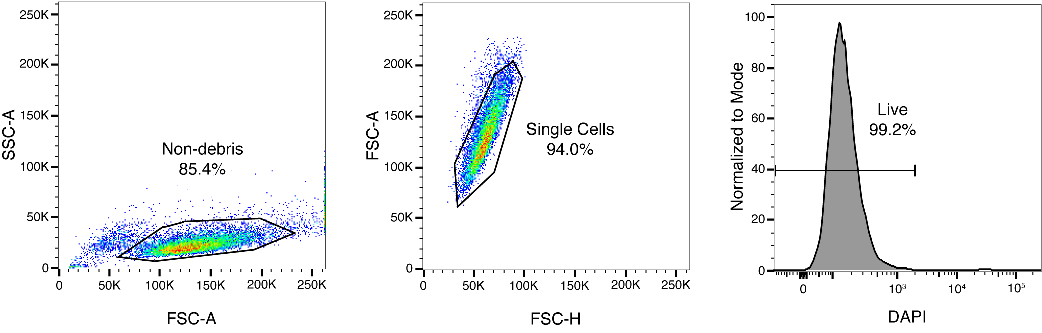
\includegraphics[keepaspectratio=true,width=\textwidth,height=\textheight]{chapters/chapter4/chapter4_SupplementaryFigure1.pdf}
    \caption{\textbf{FACS gating strategy for lectin stainings.} The cell population shown is of the parental sample shown in Figure~\ref{fig:ch4fig1}b. FSC-A: forward scatter area, SSC-A: side scatter area, FSC-H: forward scatter height.}
    \label{fig:ch4supfig1}
\end{figure}

\clearpage

\begin{figure}
    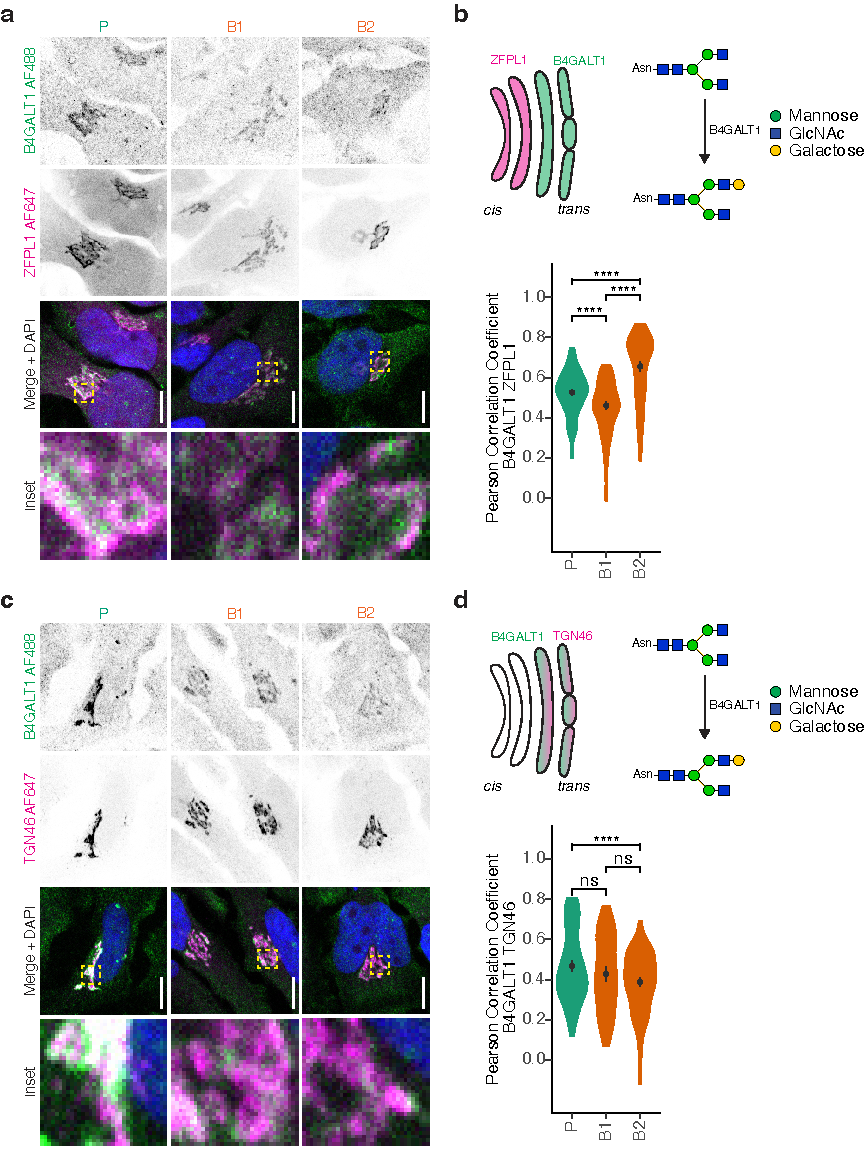
\includegraphics[keepaspectratio=true,width=\textwidth,height=\textheight]{chapters/chapter4/chapter4_SupplementaryFigure2.pdf}
    \caption{\textbf{Relocation of glycosyltransferase B4GALT1 in TMEM199KO HeLa cells.} \textbf{(a)} Immunofluorescence microscopy of B4GALT1 (green in merge) and ZFPL1 (magenta) in parental HeLa cells (green, P) or TMEM199KO cells (B1 and B2, orange). Representative confocal micrographs. Scalebars, 10 $\mu$m. DAPI in blue. \textbf{(b)} Pearson’s correlation coefficients between B4GALT1 and ZFPL1 of panel(a). N = 194 (P), 138 (B1), and 147 (B2) from two independent experiments. \textbf{(c)} Same as panel (a) but now for B4GALT1 (green) and TGN46 (magenta). \textbf{(d)} Pearson’s correlation coefficients between B4GALT1 and TGN46 of panel (c). N = 139 (P), 154 (B1), and 161 (B2) from two independent experiments.}
    \label{fig:ch4supfig2}
\end{figure}

\clearpage

\begin{figure}
    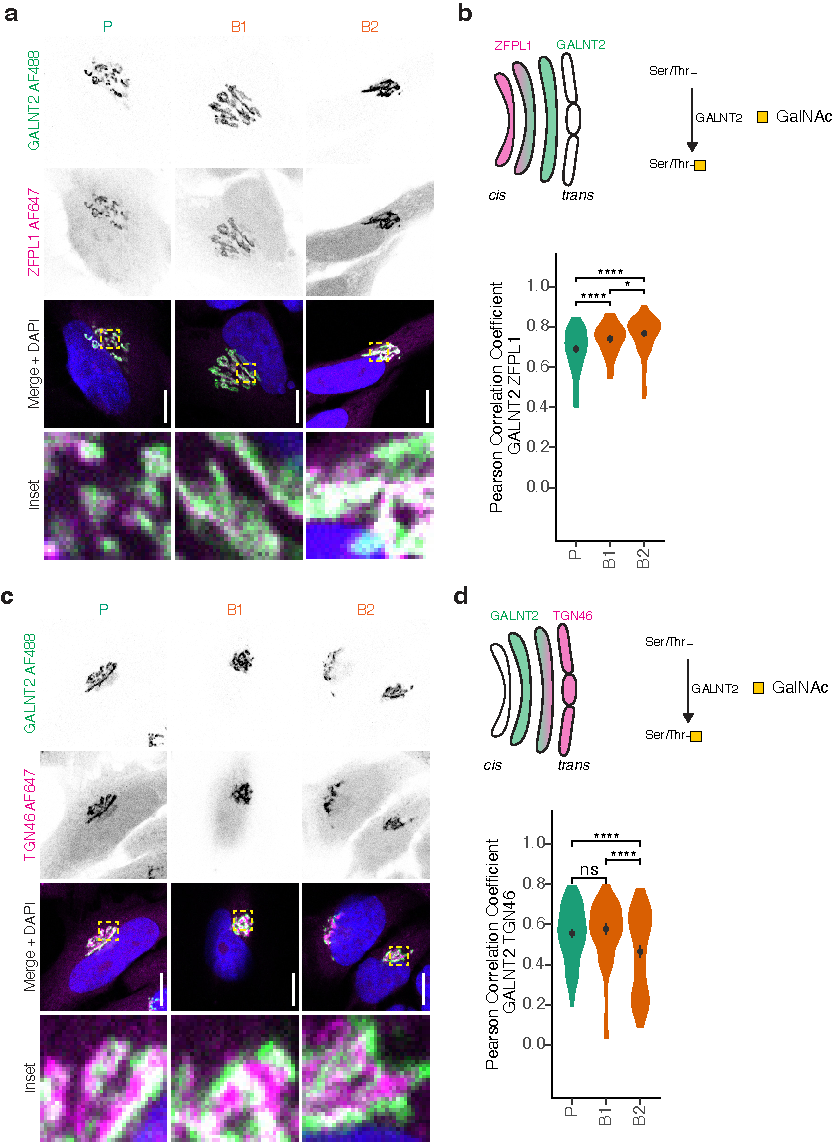
\includegraphics[keepaspectratio=true,width=\textwidth,height=\textheight]{chapters/chapter4/chapter4_SupplementaryFigure3.pdf}
    \caption{\textbf{Relocation of glycosyltransferase GALNT2 in TMEM199KO HeLa cells.} (Continued on the following page.)}
    \label{fig:ch4supfig3}
\end{figure}
\begin{figure}[t]
    \contcaption{\textbf{(a)} Immunofluorescence microscopy of GALNT2 (green in merge) and ZFPL1 (magenta) in parental HeLa cells (green, P) or TMEM199KO cells (B1 and B2, orange). Representative confocal micrographs. Scalebars, 10 $\mu$m. DAPI in blue. \textbf{(b)} Pearson’s correlation coefficients between GALNT2 and ZFPL1 of panel (a). N = 142 (P), 65 (B1), and 117 (B2) from two independent experiments. \textbf{(c)} Same as panel (a) but now for GALNT2 (green) and TGN46 (magenta). \textbf{(d)} Pearson’s correlation coefficients between GALNT2 and TGN46 of panel (c). N = 170 (P), 101 (B1), and 154 (B2) from two independent experiments.}
\end{figure}

\clearpage

\begin{figure}
    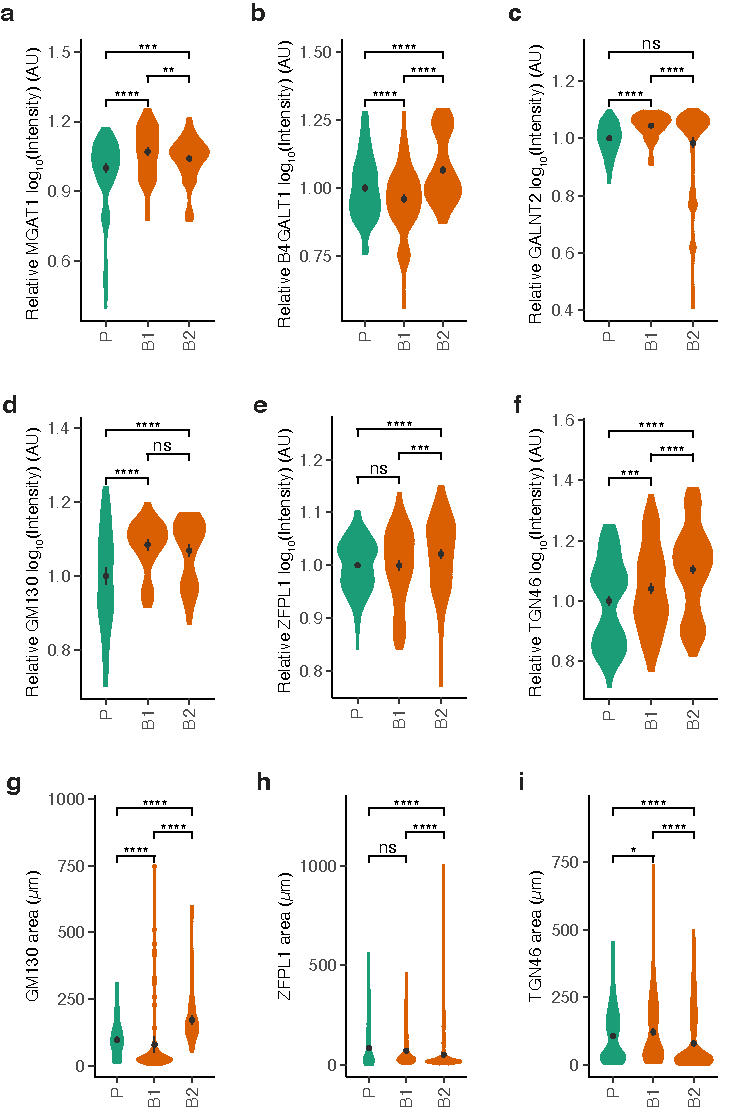
\includegraphics[keepaspectratio=true,width=\textwidth,height=\textheight]{chapters/chapter4/chapter4_SupplementaryFigure4.pdf}
    \caption{\textbf{Altered glycosyltransferase expression and Golgi morphology in TMEM199KO HeLa cells.} (Continued on the following page.)}
    \label{fig:ch4supfig4}
\end{figure}
\begin{figure}[t]
    \contcaption{\textbf{(a)} Fluorescence intensities of MGAT1 from Figure~\ref{fig:ch4fig2} relative to parental HeLa cells. N = 193 (P), 146 (B1), 198 (B2). \textbf{(b)} Same as panel (a) but now for B4GALT1 from Supplementary Figure~\ref{fig:ch4supfig2}. N = 333 (P), 226 (B1), 308 (B2). \textbf{(c)} Same as panel (a) but now for GALNT2 from Supplementary Figure~\ref{fig:ch4supfig2}. N = 312 (P), 166 (B1), 271 (B2). \textbf{(d)} Same as panel (a) but now for GM130 from Figure~\ref{fig:ch4fig2}. N = 118 (P), 78 (B1), 99 (B2). \textbf{(e)} Same as panel (a) but now for ZFPL1 from Supplementary Figures~\ref{fig:ch4supfig2} and~\ref{fig:ch4supfig3}. N = 336 (P), 203 (B1), 264 (B2). \textbf{(f)} Same as panel (a) but now for TGN46 from Figure~\ref{fig:ch4fig2} and Supplementary Figures~\ref{fig:ch4supfig2} and~\ref{fig:ch4supfig3}. N = 384 (P), 257 (B1), 414 (B2). \textbf{(g)} Quantification of GM130 fluorescence labeling area from Figure~\ref{fig:ch4fig2}. N = 118 (P), 78 (B1), 99 (B2). \textbf{(h)} Same as panel (g) but now for ZFPL1 from Supplementary Figures~\ref{fig:ch4supfig2} and~\ref{fig:ch4supfig3}. N = 336 (P), 203 (B1), 264 (B2). \textbf{(i)} Same as panel (g) but now for TGN46 from Figure~\ref{fig:ch4fig2} and Supplementary Figures~\ref{fig:ch4supfig2} and~\ref{fig:ch4supfig3}. N = 384 (P), 257 (B1), 414 (B2).}
\end{figure}

\clearpage

\begin{figure}
    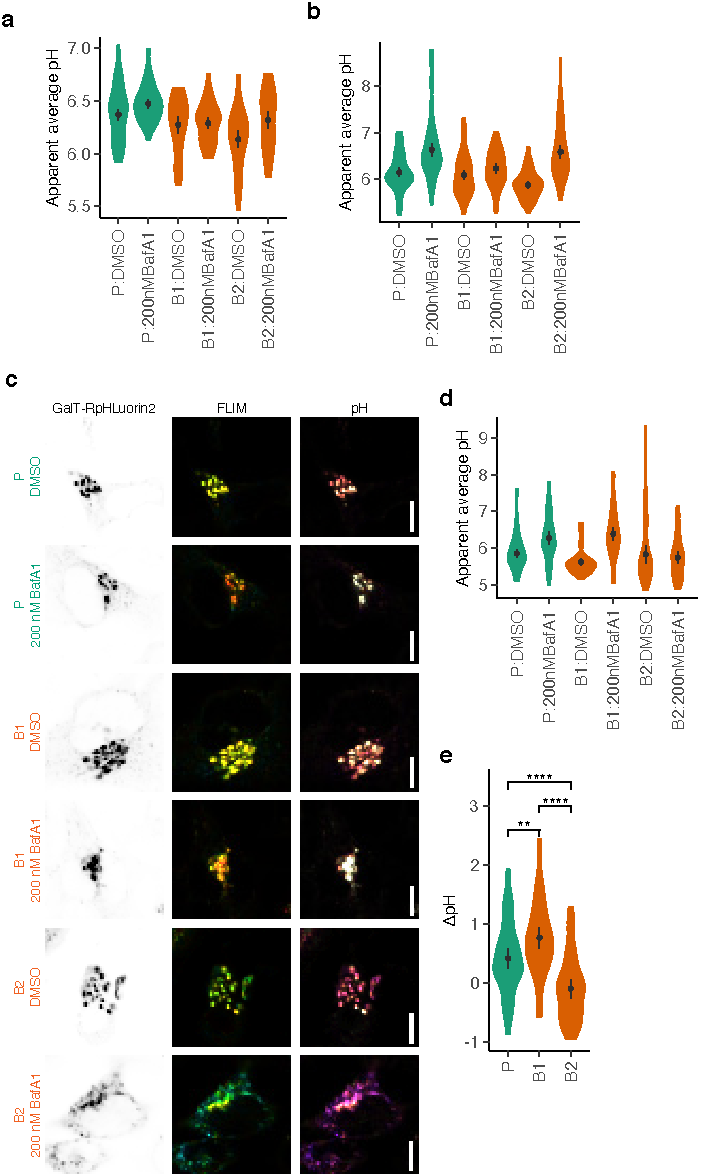
\includegraphics[keepaspectratio=true,width=\textwidth,height=\textheight]{chapters/chapter4/chapter4_SupplementaryFigure5.pdf}
    \caption{\textbf{FLIM-based pH measurements in TMEM199KO HeLa cells challenged with V-ATPase inhibitor Bafilomycin A1.} (Continued on the following page.)}
    \label{fig:ch4supfig5}
\end{figure}
\begin{figure}[t]
    \contcaption{\textbf{(a)} Full quantification of pH from Figure~\ref{fig:ch4fig4}a. The values presented here were used to generate the $\Delta$pH plot. \textbf{(b)} Same as panel (a) but now for Figure~\ref{fig:ch4fig4}c. \textbf{(c)} Representative confocal micrographs of parental HeLa cells (P, green) or TMEM199KO cells (B1 and B2, orange) expressing GalT-RpHLuorin2, in the absence (DMSO) or presence of Bafilomycin A1 (200 nM BafA1). The intensity image (left column) was convoluted with the fluorescence lifetime value (middle column) and the calculated pH (right column) per pixel. FLIM, fluorescence lifetime imaging microscopy. Scalebars, 10 $\mu$m. \textbf{(d)} Same as panel (a) but now for panel (c). \textbf{(e)} Quantification of the difference in pH ($\Delta$pH) between vehicle control (DMSO) and cells challenged with Bafilomycin A1 from panel (c). N = 68 (P, DMSO), 50 (P, 200 nM BafA1), 48 (B1, DMSO), 49 (B1, 200 nM BafA1), 46 (B2, DMSO), and 44 (B2, 200 nM BafA1) from 2 independent experiments.}
\end{figure}
